\chapter{Malware Detection}

\section{YARA}

\subsection{Lab01-01}

\textbf{Rilevamento di Lab01-01.dll}:

Il primo task ha richiesto l'estrazione di indicatori basati sull'host all'interno della libreria dinamica. Tramite la finestra delle stringhe di IDA Pro (e la verifica delle chiamate all'interno di \texttt{DllMain}), sono stati identificati i seguenti IoC:

\begin{figure}[H]
  \centering
  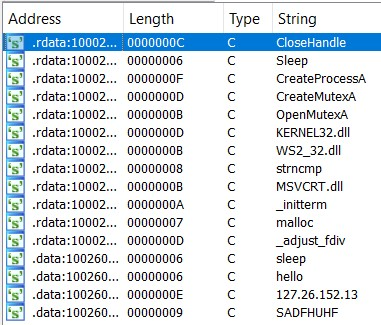
\includegraphics[width=0.7\textwidth]{../8.MalwareDetection/img/stringhe_dll.jpg}
  \caption{Stringhe estratte da \texttt{Lab01-01.dll} in IDA Pro}
\end{figure}

\begin{figure}[H]
  \centering
  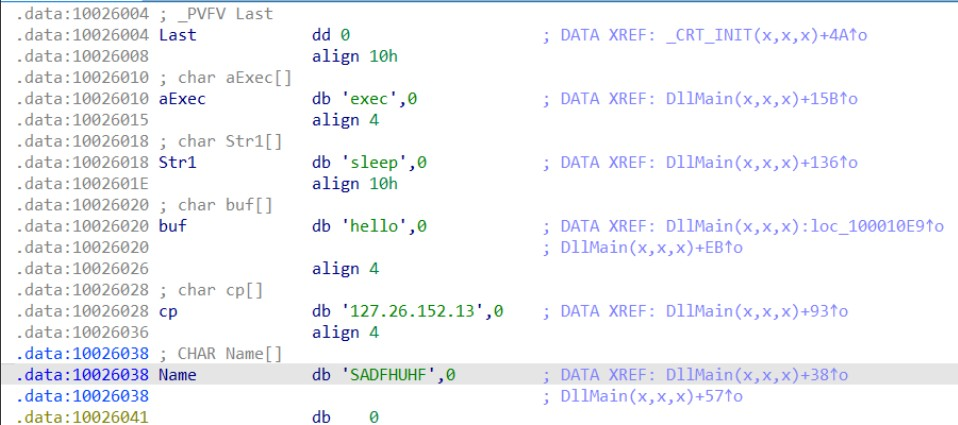
\includegraphics[width=0.7\textwidth]{../8.MalwareDetection/img/stringhe_dll_spec.jpg}
  \caption{Dettaglio delle stringhe di rete e comandi}
\end{figure}

Indirizzo IP Hardcoded: \texttt{127.26.152.13}, inserito nello stack prima di specifiche esecuzioni.

\begin{figure}[H]
  \centering
  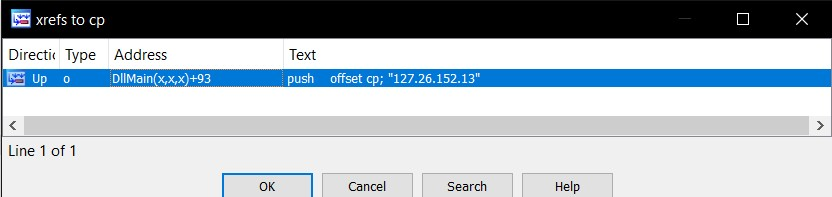
\includegraphics[width=0.7\textwidth]{../8.MalwareDetection/img/stringhe_dll_pos_cp.jpg}
  \caption{Caricamento dell'indirizzo IP locale nello stack}
\end{figure}

Nome del Mutex: \texttt{SADFHUHF}, stringa specifica associata alla creazione e apertura di mutex (\texttt{CreateMutexA}, \texttt{OpenMutexA}) per garantire l'esecuzione di una singola istanza del malware.

\begin{figure}[H]
  \centering
  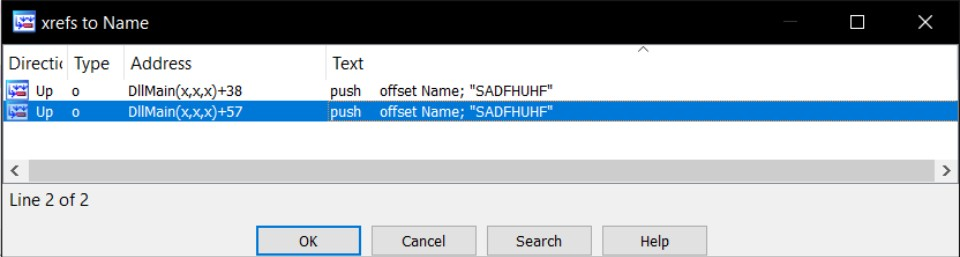
\includegraphics[width=0.7\textwidth]{../8.MalwareDetection/img/stringhe_dll_pos_name.jpg}
  \caption{Riferimento alla stringa del Mutex in IDA Pro}
\end{figure}

Comandi aggiuntivi: Stringhe in chiaro come \texttt{hello}, \texttt{exec} e \texttt{sleep}.

La regola YARA è stata strutturata per scattare qualora vengano individuate almeno due di queste specifiche stringhe all'interno del file analizzato.

Snippet di codice:
\begin{lstlisting}
rule Lab01_01_DLL {
    meta:
        description = "Rilevamento di Lab01-01.dll basato su Mutex e IP"
        author = "Il tuo nome"
    
    strings:
        $mutex = "SADFHUHF"
        $ip = "127.26.152.13"
        $cmd_hello = "hello"
        $cmd_exec = "exec"
        $cmd_sleep = "sleep"

    condition:
        2 of ($mutex, $ip, $cmd_hello, $cmd_exec, $cmd_sleep)
}
\end{lstlisting}

\begin{figure}[H]
  \centering
  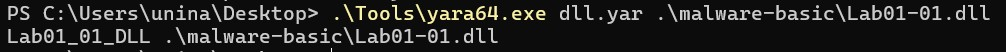
\includegraphics[width=0.7\textwidth]{../8.MalwareDetection/img/stringhe_dll_res.jpg}
  \caption{Risultato del rilevamento YARA per la DLL}
\end{figure}

\textbf{Rilevamento di Lab01-01.exe}:

Il secondo task si è concentrato sul file eseguibile principale. L'ispezione con IDA Pro ha portato all'individuazione di due artefatti critici:

\begin{figure}[H]
  \centering
  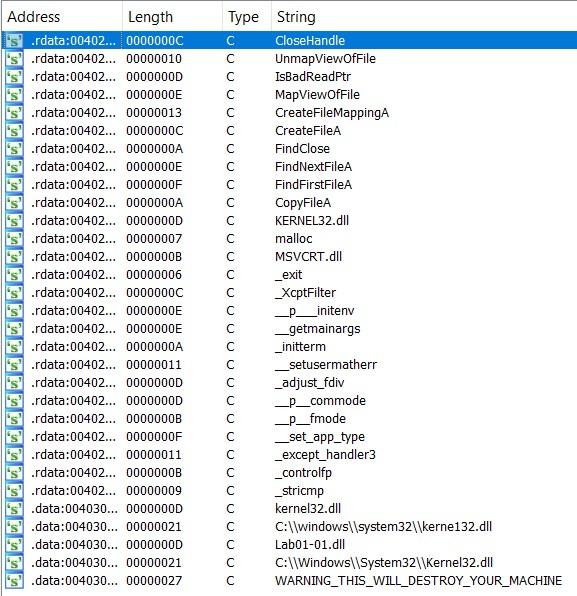
\includegraphics[width=0.7\textwidth]{../8.MalwareDetection/img/stringhe_exe.jpg}
  \caption{Stringhe estratte da \texttt{Lab01-01.exe} in IDA Pro}
\end{figure}

\begin{figure}[H]
  \centering
  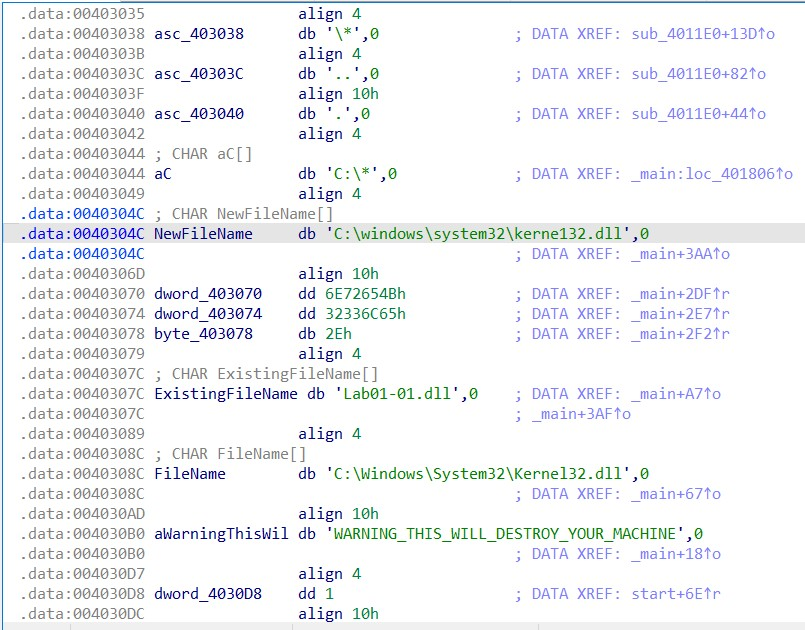
\includegraphics[width=0.7\textwidth]{../8.MalwareDetection/img/stringhe_exe_spec.jpg}
  \caption{Dettaglio delle stringhe e librerie importate dall'eseguibile}
\end{figure}

Percorso DLL Malevola: Un percorso di sistema alterato, utilizzato presumibilmente per caricare la libreria nociva mascherandola da processo legittimo.

\begin{figure}[H]
  \centering
  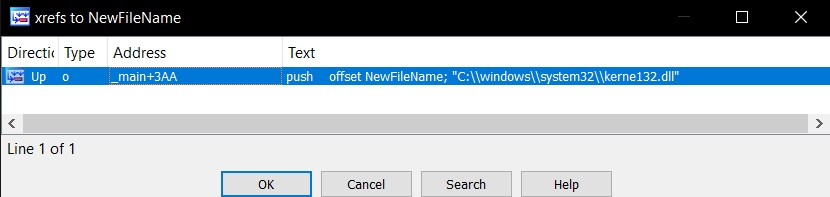
\includegraphics[width=0.7\textwidth]{../8.MalwareDetection/img/stringhe_exe_pos_newfilename.jpg}
  \caption{Locazione del percorso del file di typosquatting \texttt{kerne132.dll}}
\end{figure}

Messaggio di Testo: Una stringa di avviso hardcoded stampata a schermo dal malware.

\begin{figure}[H]
  \centering
  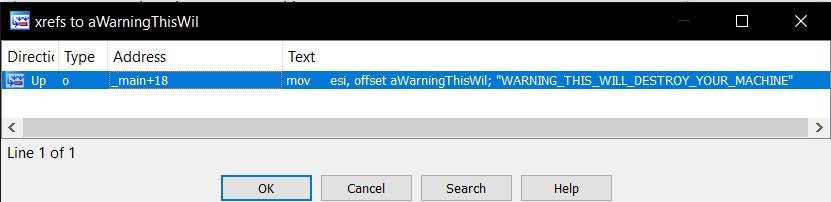
\includegraphics[width=0.7\textwidth]{../8.MalwareDetection/img/stringhe_exe_pos_warn.jpg}
  \caption{Riferimento alla stringa di WARNING}
\end{figure}

Snippet di codice:
\begin{lstlisting}
rule Lab01_01_EXE {
    meta:
        description = "Rilevamento di Lab01-01.exe"
        author = "Il tuo nome"
    
    strings:
        $dll_path = "C:\\windows\\system32\\kerne132.dll" 
        $message = "WARNING_THIS_WILL_DESTROY_YOUR_MACHINE" 

    condition:
        all of them
}
\end{lstlisting}

\begin{figure}[H]
  \centering
  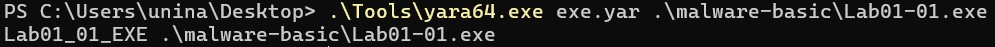
\includegraphics[width=0.7\textwidth]{../8.MalwareDetection/img/stringhe_exe_res.jpg}
  \caption{Risultato del rilevamento YARA per l'eseguibile}
\end{figure}

\subsection{Lab01-04}

Durante l'ispezione iniziale con il disassemblatore IDA Pro, l'analisi strutturale standard ha evidenziato la presenza di chiamate a funzioni di gestione delle risorse di Windows (quali \texttt{FindResourceA}, \texttt{LoadResource} e \texttt{SizeofResource}).

\begin{figure}[H]
  \centering
  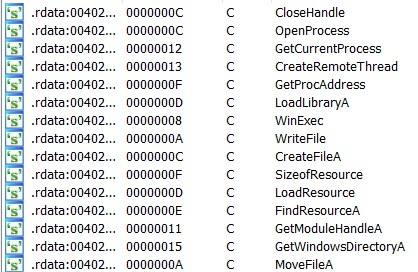
\includegraphics[width=0.7\textwidth]{../8.MalwareDetection/img/stringhe_4_1.jpg}
  \caption{Funzioni di gestione risorse utilizzate nel codice}
\end{figure}

\begin{figure}[H]
  \centering
  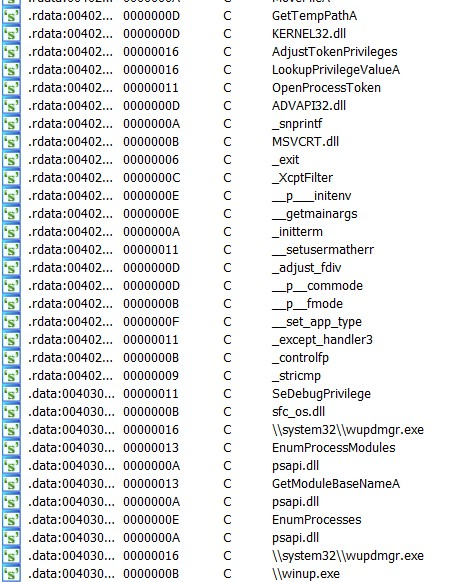
\includegraphics[width=0.7\textwidth]{../8.MalwareDetection/img/stringhe_4_2.jpg}
  \caption{Visualizzazione grafica del flusso di caricamento risorse}
\end{figure}

\begin{figure}[H]
  \centering
  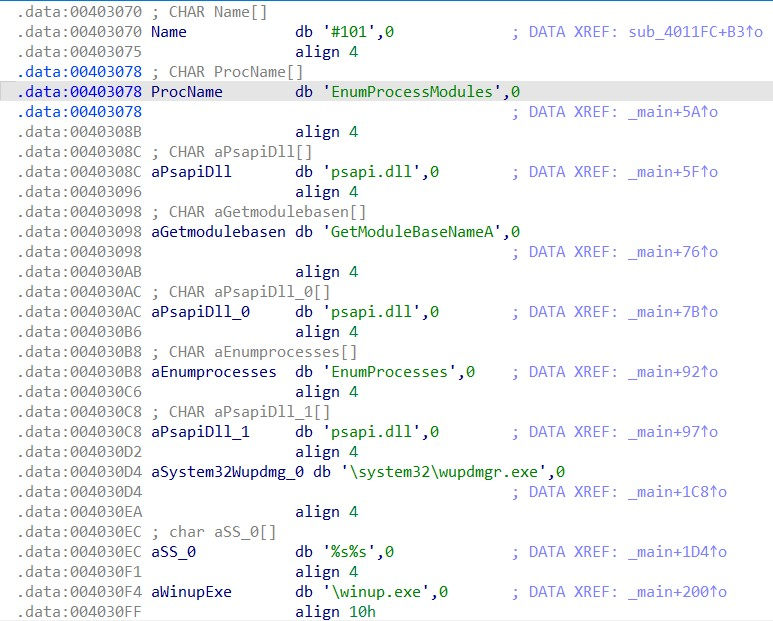
\includegraphics[width=0.7\textwidth]{../8.MalwareDetection/img/stringhe_4_spec.jpg}
  \caption{Parametri di \texttt{FindResourceA} indicanti l'estrazione di un eseguibile secondario}
\end{figure}

Questa configurazione è tipica dei dropper, ovvero programmi malevoli che fungono da contenitori e che occultano un secondo payload eseguibile all'interno della propria sezione risorse (\texttt{.rsrc}).
A causa di questo incapsulamento, la vista standard delle stringhe di IDA Pro non è stata in grado di indicizzare o mostrare direttamente il dominio di comando e controllo cercato. È stato quindi necessario adottare un approccio alternativo basato sulla scansione dei byte grezzi tramite \texttt{yarGen} per estrarre gli indicatori nascosti.

\begin{figure}[H]
  \centering
  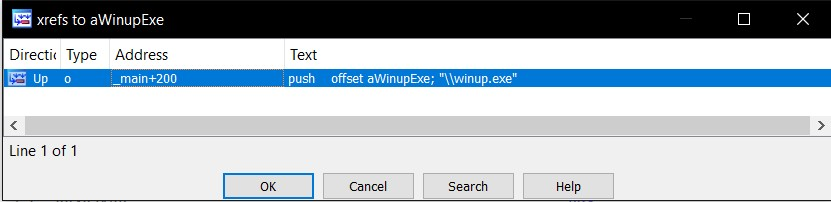
\includegraphics[width=0.7\textwidth]{../8.MalwareDetection/img/stringhe_4_winup_pos.jpg}
  \caption{Riferimento alla stringa \texttt{\textbackslash winup.exe} all'interno delle risorse grezze}
\end{figure}

\begin{figure}[H]
  \centering
  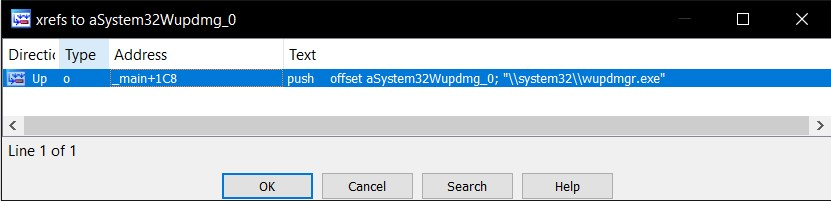
\includegraphics[width=0.7\textwidth]{../8.MalwareDetection/img/stringhe_4_wupd_pos.jpg}
  \caption{Identificazione dell'URL del dominio C2 e di \texttt{\textbackslash wupdmgr.exe}}
\end{figure}

Lanciando lo strumento \texttt{yarGen} con il database di goodware abilitato per filtrare le stringhe legittime del sistema operativo, è stata estratta una firma euristica iniziale che ha esposto con successo tutti gli artefatti annidati all'interno della risorsa binaria. Di seguito viene riportata l'esatta struttura della regola YARA generata automaticamente dal tool:

\begin{lstlisting}
rule Lab01_04 {
   meta:
      description = "malware-basic - file Lab01-04.exe"
      author = "yarGen Rule Generator"
      reference = "https://github.com/Neo23x0/yarGen"
      date = "2026-06-10"
      hash1 = "0fa1498340fca6c562cfa389ad3e93395f44c72fd128d7ba08579a69aaf3b126"
   strings:
      $s1 = "\\system32\\wupdmgrd.exe" fullword ascii
      $s2 = "\\system32\\wupdmgr.exe" fullword ascii
      $s3 = "http://www.practicalmalwareanalysis.com/updater.exe" fullword ascii
      $s4 = "\\winup.exe" fullword ascii
      $s5 = "<not real>" fullword ascii
   condition:
      uint16(0) == 0x5a4d and filesize < 100KB and
      all of them
}
\end{lstlisting}

Analizzando la regola grezza sopra riportata, emergono le seguenti considerazioni ingegneristiche:
La dicitura \texttt{uint16(0) == 0x5a4d} verifica l'intestazione logica del file (``MZ'' tipico dei Portable Executable di Windows), mentre \texttt{filesize < 100KB} impedisce al motore YARA di saturare le risorse di calcolo scansionando file massivi non pertinenti.

Le stringhe \texttt{\$s2} (\texttt{\textbackslash system32\textbackslash wupdmgr.exe}), \texttt{\$s3} (il dominio C2 \texttt{http://www...}) e \texttt{\$s4} (\texttt{\textbackslash winup.exe}) costituiscono l'impronta comportamentale univoca del malware. Esse descrivono il tentativo del dropper di sovrascrivere il Windows Update Manager originale con un binario malevolo.

La stringa \texttt{\$s5 = "<not real>"} rappresenta un artefatto volatile o un potenziale elemento di disturbo. Se l'attaccante decidesse di ricompilare il codice modificando o rimuovendo questa stringa inerte, la regola YARA strutturata con la condizione \texttt{all of them} fallirebbe l'identificazione, generando un falso negativo. È quindi imperativo rimuoverla.

I nomi generici assegnati alle variabili (\texttt{\$s1}, \texttt{\$s2}, ecc.) riducono la scannabilità del codice per i team di Incident Response. È opportuno rinominare le variabili con identificativi semantici chiari.

Applicando i criteri di raffinamento descritti, la regola è stata reingegnerizzata per mantenere la massima reattività e azzerare le possibilità di elusione basate su stringhe non operative:

\begin{lstlisting}
rule Lab01_04_EXE_Refined {
    meta:
        description = "malware-basic - file Lab01-04.exe"
    
    strings:
        // Indicatori host: percorsi dei file binari scritti o manipolati dal dropper
        $path_wupdmgr = "\\system32\\wupdmgr.exe" fullword ascii
        $path_winup   = "\\winup.exe" fullword ascii
        
        // Indicatore di rete: dominio C2 hardcoded estratto dalle risorse grezze
        $c2_url       = "http://www.practicalmalwareanalysis.com/updater.exe" fullword ascii

    condition:
        // Vincoli strutturali del file PE uniti alla presenza degli IoC
        uint16(0) == 0x5a4d and 
        filesize < 100KB and 
        all of ($path_wupdmgr, $path_winup, $c2_url)
}
\end{lstlisting}

\begin{figure}[H]
  \centering
  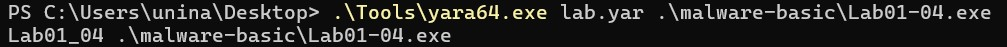
\includegraphics[width=0.7\textwidth]{../8.MalwareDetection/img/stringhe_4_res.jpg}
  \caption{Risultato del rilevamento YARA con la regola raffinata}
\end{figure}

\section{Astaroth}

Astaroth è un Trojan altamente sofisticato specializzato nel furto di credenziali. La sua particolarità risiede nell'esteso utilizzo di tecniche fileless e nell'abuso di LOLBins (Living Off The Land Binaries). Invece di scaricare binari eseguibili sospetti, Astaroth sfrutta utility legittime preinstallate in Windows (come \texttt{bitsadmin.exe}, \texttt{cmd.exe} ed \texttt{extexport.exe}) per bypassare i controlli perimetrali, decifrare i propri payload e garantirsi la persistenza nel sistema senza allertare le soluzioni antivirus tradizionali.

Per monitorare l'attività del malware è stato impiegato Sysmon (System Monitor), focalizzando l'analisi sui seguenti identificatori:

\begin{itemize}
  \item \textbf{EventID 1 (Process Create)}: Per tracciare l'esecuzione dei LOLBins e i parametri passati a riga di comando.
  \item \textbf{EventID 11 (File Create)}: Per intercettare la scrittura di payload o file di collegamento (\texttt{.lnk}) nelle cartelle di esecuzione automatica.
  \item \textbf{EventID 12 (Registry Event)}: Per monitorare la manomissione delle chiavi di registro legate alla persistenza al boot.
\end{itemize}

È stato sviluppato un set completo di 6 regole Sigma in formato YAML.

\begin{itemize}
  \item \textbf{\texttt{astaroth-bits.yml}}: Intercetta l'avvio di \texttt{bitsadmin.exe} associato a flag di copia o trasferimento (\texttt{/transfer}). Questo tool viene abusato dallo stager iniziale per scaricare i payload dal server C2 (Command \& Control).
\begin{lstlisting}[language=XML]
title: Bitsadmin Download
id: d059842b-6b9d-4ed1-b5c3-5b89143c6ede
status: experimental
description: Detects usage of bitsadmin downloading a file
references:
  - https://blog.netspi.com/15-ways-to-download-a-file/#bitsadmin
  - https://isc.sans.edu/diary/22264
tags:
  - attack.defense_evasion
  - attack.persistence
  - attack.t1197
  - attack.s0190
date: 2017/03/09
modified: 2019/12/06
author: Michael Haag
logsource:
  product: windows
  service: sysmon
detection:
  event:
    EventID: 1
  selection1:
    Image: '*\bitsadmin.exe'
    CommandLine: '* /transfer *'
  selection2:
    CommandLine: '*copy *bitsadmin.exe*'
  condition: event and (selection1 or selection2)
fields:
  - CommandLine
  - ParentCommandLine
falsepositives:
  - Some legitimate apps use this, but limited.
level: medium
\end{lstlisting}

  \item \textbf{\texttt{astaroth-extexport.yml}}: Rileva l'esecuzione di \texttt{extexport.exe} al di fuori dei percorsi canonici di Internet Explorer. Questo binario viene tipicamente forzato da Astaroth per eseguire DLL malevole tramite la tecnica del DLL Side-Loading.
\begin{lstlisting}[language=XML]
title: ExtExport.exe DLL Side Loading
id: a1b2c3d4-e5f6-7a8b-9c0d-1e2f3a4b5c6d
status: experimental
description: Detects ExtExport.exe execution indicating a DLL Side-Loading attempt.
references:
  - https://lolbas-project.github.io/lolbas/Binaries/Extexport/
tags:
  - attack.execution
  - attack.defense_evasion
  - attack.t1059
  - attack.t1073
author: Martin, Anartz
date: 2020/06/30
logsource:
  product: windows
  service: sysmon
detection:
  selection:
    EventID: 1
    Image: '*\extexport.exe'
  filter:
    CommandLine:
      - '^[Cc]:\\[Pp]rogram\ [Ff]iles(\ \([Xx]86\))?\\([Ii]nternet\ [Ee]xplorer\\[Ee]xt[Ee]xport\.exe$'
  condition: selection and not filter
fields:
  - CommandLine
falsepositives:
  - Depending on the estate activity. They should be rare.
level: medium
\end{lstlisting}

  \item \textbf{\texttt{astaroth-reg.yml}}: Regola specifica che rileva la manipolazione (\texttt{EventType: DeleteValue}) della chiave Shell Folders all'interno dell'alveare di registro esatto dell'utente del laboratorio (\texttt{HKU\textbackslash S-1-5-21...}).
\begin{lstlisting}[language=XML]
title: Add Startup Key to Explorer Shell Folders
id: e2a9c7a3-5b2a-4b7e-a8b2-4de0f6e8a6cd
status: experimental
description: Detects the insert of a registry value
references:
  - https://example.com/reference1
  - https://example.com/reference2
tags:
  - attack.defense_evasion
  - attack.persistence
  - attack.t1112
  - attack.s0190
logsource:
  product: windows
  service: sysmon
detection:
  selection:
    EventID: 12
    Image: 'C:\Windows\System32\cmd.exe'
    EventType: 'DeleteValue'
    TargetObject: 'HKU\S-1-5-21-3191581004-3819144844-3633199379-1002\SOFTWARE\Microsoft\Windows\*'
  condition: selection
fields:
  - UtcTime
  - ProcessGuid
  - ProcessId
  - Image
  - TargetObject
  - User
falsepositives:
  - Legitimate administrative actions
level: medium
\end{lstlisting}

  \item \textbf{\texttt{astaroth-reg-modify.yml}}: Regola generica che intercetta la creazione di un processo (EventID 1) associato a \texttt{reg.exe} la cui riga di comando contenga la stringa ``Shell Folders''.
\begin{lstlisting}[language=XML]
title: Astaroth Generic Registry Modification
description: "Detects process creation events using reg.exe to modify Shell Folders."
id: "b1111111-2222-3333-4444-555555555555"
tags:
  - attack.persistence
logsource:
  product: windows
  service: sysmon
detection:
  selection:
    EventID: 1
    CommandLine|contains|all:
      - 'reg.exe'
      - 'Shell Folders'
  condition: selection
level: high
\end{lstlisting}

  \item \textbf{\texttt{astaroth-startup.yml}}: Regola specifica (EventID 11) che traccia il momento in cui \texttt{cmd.exe} tenta di creare fisicamente il file \texttt{launcher.lnk} nel percorso assoluto di esecuzione automatica dell'utente unina.
\begin{lstlisting}[language=XML]
title: File Creation by CMD in Startup Folder
id: a3b4c8e3-7f2a-4d7e-b2c5-8e6f8b8d7fcd
status: experimental
description: Detects the creation of a file in the startup folder by cmd.exe
references:
  - https://example.com/reference1
  - https://example.com/reference2
tags:
  - attack.persistence
  - attack.t1547.001
  - attack.s0190
logsource:
  product: windows
  service: sysmon
detection:
  selection:
    EventID: 11
    Image: 'C:\Windows\System32\cmd.exe'
    TargetFilename: 'C:\Users\unina\AppData\Roaming\Microsoft\Windows\Start Menu\Programs\Startup\launcher.lnk'
  condition: selection
fields:
  - UtcTime
  - ProcessGuid
  - ProcessId
  - Image
  - TargetFilename
  - User
falsepositives:
  - Legitimate administrative actions or script usage
level: critical
\end{lstlisting}

  \item \textbf{\texttt{astaroth-startup-detection.yml}}: Regola generica che segnala qualsiasi file con estensione eseguibile (\texttt{.lnk}, \texttt{.bat}, \texttt{.ps1}, \texttt{.exe}) creato all'interno della directory globale o utente di Startup.
\begin{lstlisting}[language=XML]
title: Start-up Detection
description: Detects generic file creation in the Startup folder with executable extensions.
id: "c1111111-2222-3333-4444-555555555555"
tags:
  - attack.persistence
logsource:
  product: windows
  service: sysmon
detection:
  selection:
    EventID: 11
    TargetFilename|contains: '\Start Menu\Programs\Startup\'
    TargetFilename|endswith:
      - '.lnk'
      - '.bat'
      - '.ps1'
      - '.exe'
  condition: selection
level: high
\end{lstlisting}
\end{itemize}

Di seguito è stato eseguito ZircoLite per verificare l'efficacia delle regole analizzando i log generati da Sysmon:

\begin{figure}[H]
  \centering
  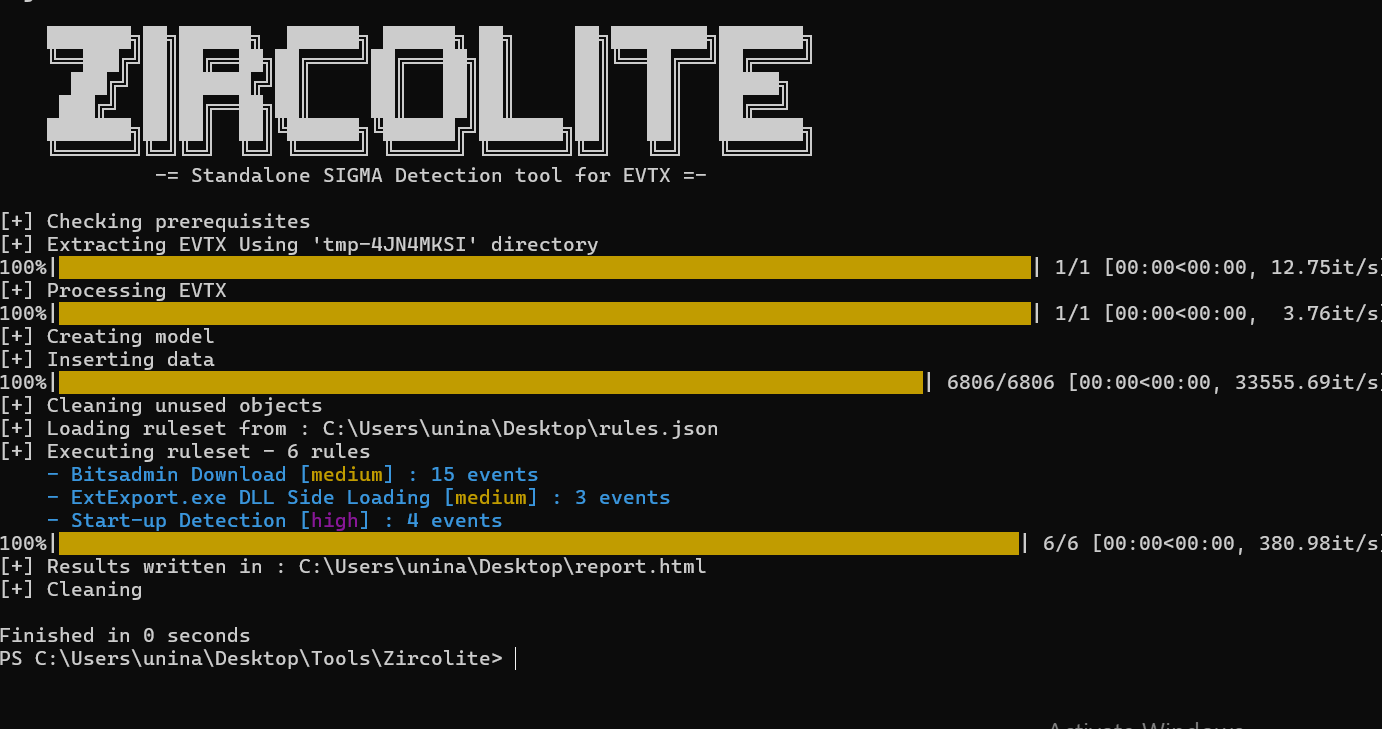
\includegraphics[width=0.7\textwidth]{../8.MalwareDetection/img/zircolite_success.png}
  \caption{Esecuzione riuscita di ZircoLite con regole personalizzate}
\end{figure}

Il comando ZircoLite eseguito è il seguente:
\begin{lstlisting}[language=bash]
python .\zircolite.py --evtx "C:\Users\unina\Desktop\sysmon_log.evtx" --ruleset "C:\Users\unina\Desktop\rules_astaroth.json"
\end{lstlisting}

\section{SNORT}

Il malware è progettato per infettare l'host, raccogliere informazioni identificative sul sistema compromesso e avviare una comunicazione silente (beaconing) verso un server di Command \& Control (C2) per segnalare il successo dell'infezione.

L'analisi dinamica, condotta isolando il campione ed eseguendolo in un ambiente controllato tramite FakeNet-NG, ha rivelato il seguente comportamento di rete:

\begin{figure}[H]
  \centering
  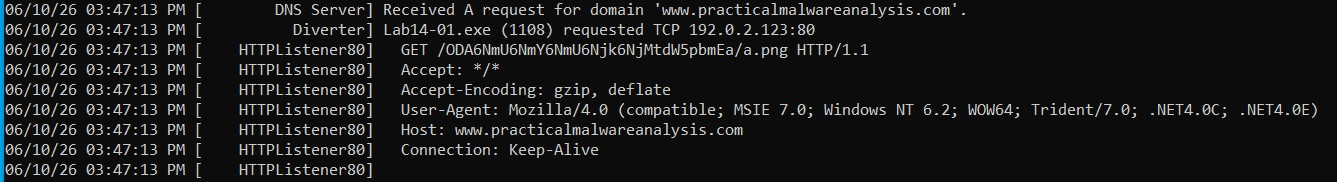
\includegraphics[width=0.7\textwidth]{../8.MalwareDetection/img/snort-connection.jpg}
  \caption{Richieste di beaconing intercettate in rete}
\end{figure}

\begin{itemize}
  \item \textbf{Librerie di Rete Utilizzate}: Il malware fa uso delle librerie di rete standard di Windows (come le API WinINet). Questo gli permette di generare richieste HTTP strutturalmente perfette, ereditando gli header di sistema (es. \texttt{Accept-Encoding: gzip, deflate}) per mimetizzarsi nel normale traffico web.
  \item \textbf{Tecnica di Mascheramento}: Utilizza un'intestazione User-Agent contraffatta ma valida (\texttt{Mozilla/4.0 (compatible; MSIE 7.0; Windows NT 6.2; WOW64; Trident/7.0; .NET4.0C; .NET4.0E)}). Questo simula il traffico generato da un vecchio browser Internet Explorer, rendendo difficile l'individuazione tramite ispezioni superficiali.
  \item \textbf{Dati Esfiltrati}: Il malware ruba due parametri fondamentali: l'Hardware Profile GUID (letto dal registro di sistema) e il Nome Utente della sessione corrente. Queste informazioni permettono all'attaccante di identificare univocamente le vittime ed evitare conteggi doppi nella botnet.
  \item \textbf{Codifica e Trasmissione}: I dati non sono cifrati, ma codificati utilizzando lo standard Base64 (es. \texttt{80:6e:6f:6e:69:63-unina} diventa \texttt{ODA6NmU6NmY6NmU6Njk6NjMtdW5pbmEa}). Questa stringa viene poi inserita direttamente nell'URI di una richiesta HTTP GET.
\end{itemize}

La creazione della regola di rilevamento ha richiesto l'identificazione degli Indicatori di Compromissione (IoC) corretti, evitando le classiche trappole che generano falsi allarmi o mancate rilevazioni.

\textbf{Errori da evitare}:
\begin{itemize}
  \item \textbf{Falsi Positivi}: Non è possibile utilizzare lo User-Agent come trigger per l'allarme. Trattandosi di una stringa legittima di Internet Explorer, la regola bloccherebbe il traffico web di macchine non aggiornate.
  \item \textbf{Falsi Negativi (Hardcoding)}: Non è possibile cercare la stringa Base64 esatta, poiché variando l'Hardware ID e l'utente, la stringa muterà per ogni singola infezione. Inoltre, l'analisi dinamica ha dimostrato che il nome del file immagine richiesto varia dinamicamente (es. \texttt{y.png}, \texttt{a.png}).
\end{itemize}

\textbf{Indicatori Affidabili scelti per la Regola}:
\begin{itemize}
  \item Dominio C2 (Host): \texttt{www.practicalmalwareanalysis.com}
  \item Pattern dell'URI (PCRE): Una struttura composta da \texttt{/} + [Stringa Base64] + \texttt{/} + [singola lettera casuale] + \texttt{.png}.
\end{itemize}

\textbf{Regola Snort Definitiva} per rilevamento beaconing del malware:

\begin{lstlisting}
alert tcp $HOME_NET any -> $EXTERNAL_NET $HTTP_PORTS ( \
    msg:"ET MALWARE Lab14-01 Beaconing Detected"; \
    flow:established,to_server; \
    content:"GET"; http_method; \
    content:"www.practicalmalwareanalysis.com"; http_header; \
    pcre:"/^\/[A-Za-z0-9+\/=]+\/[a-z]\.png$/U"; \
    classtype:trojan-activity; \
    sid:1000014; rev:1; \
)
\end{lstlisting}

Per intercettare varianti in cui l'attaccante ha semplicemente cambiato il dominio di destinazione, è necessaria una regola euristica che ometta l'host ma irrigidisca l'espressione regolare (richiedendo un Base64 di almeno 15 caratteri, numero abbastanza alto da tagliare fuori la maggior parte del traffico web legittimo, ma sufficientemente basso da non farsi sfuggire il malware nel caso infettasse un PC con un nome utente corto) per evitare falsi positivi:

\begin{lstlisting}
alert tcp $HOME_NET any -> $EXTERNAL_NET $HTTP_PORTS ( \
    msg:"ET MALWARE Generic Base64 PNG Beaconing Pattern"; \
    flow:established,to_server; \
    content:"GET"; http_method; \
    content:".png"; http_uri; fast_pattern; \
    pcre:"/^\/[A-Za-z0-9+\/=]{15,}\/[a-z]\.png$/U"; \
    classtype:trojan-activity; \
    sid:1000015; rev:1; \
)
\end{lstlisting}

Per garantire che le varianti future di questo malware vengano bloccate (ad esempio nel caso l'attaccante modifichi il dominio o la struttura dell'URI), è necessario implementare un set di firme multilivello (Defense in Depth):

\begin{itemize}
  \item \textbf{Firme di Rete (Network Signatures)}: Implementazione della regola Snort descritta sopra, unita al blocco DNS per il dominio malevolo noto.
  \item \textbf{Firme di Host (YARA)}: Creazione di firme statiche basate sull'analisi in IDA Pro per rilevare la presenza di combinazioni specifiche di API importate (es. importazione contemporanea di \texttt{WinINet.dll}, \texttt{GetUserNameA} e manipolazione di \texttt{HwProfileGuid}).
  \item \textbf{Firme Comportamentali (Sigma/Sysmon)}: Creazione di regole per rilevare i processi non autorizzati che tentano di accedere alla chiave di registro \texttt{HKLM\textbackslash System\textbackslash CurrentControlSet\textbackslash Control\textbackslash IDConfigDB\textbackslash Hardware Profiles}.
\end{itemize}
